\section{Caso Pr�ctico}

	En este cap�tulo se presenta un ejemplo concreto de la propuesta, para lo cual se reutilizar� la simulaci�n que forma parte del proyecto ZNN.
	El sistema consiste en sitio de noticias y la simulaci�n nos permite manejar variables tales como la cantidad de servidores, la fidelidad de la informaci�n que se provee, o sea, permite eliminar determinado tipo de contenido (e.g: videos) para mejorar el tiempo de respuesta experimentado por el usuario del sitio.
	
	Comenzaremos considerando c�mo se comporta el sistema al no existir escenarios ni estrategias, esto nos permitir� evaluar la variaci�n de comportamiento al ir agregando escenarios.
	Para simplificar el ejemplo, los datos que nos interesar�n ser�n el tiempo de respuesta experimentado por el usuario y el costo de servidores del sistema, que para simplificar reflejar� simplemente la cantidad de servidores levantados con que cuenta el sistema en cada momento.
	
	Entonces, el comportamiento del sistema sin escenarios, o sea, sin autoreparaci�n ser� el siguiente:

	\begin{center}
		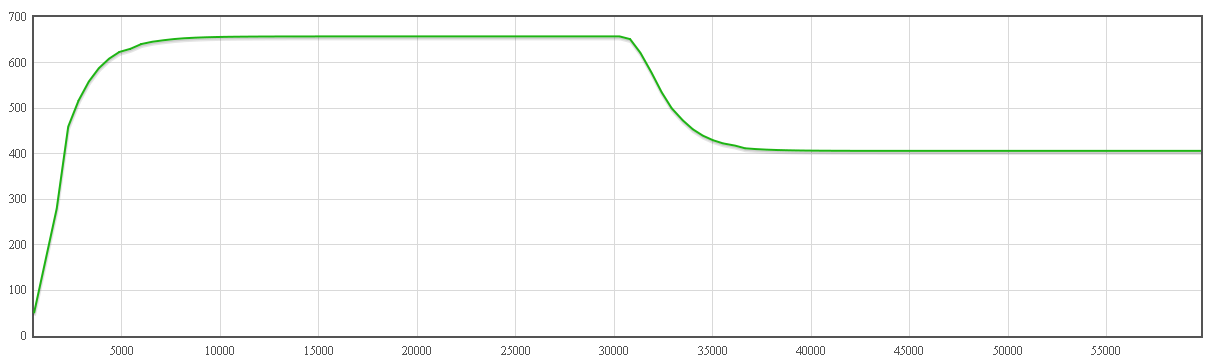
\includegraphics{images/testcase1_1_expRespTime.png}
	\end{center}

	\begin{center}
		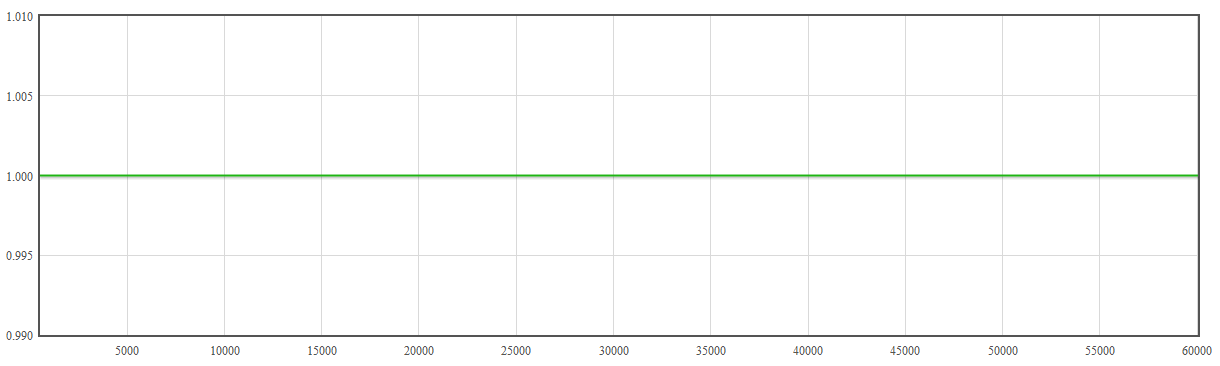
\includegraphics{images/testcase1_1_cost.png}
	\end{center}

	Como podemos observar, el tiempo de respuesta crece hasta superar los 600ms, manteni�ndose as� por unos 10 segundos, luego el mismo va bajando escalonadamente hasta estacionarse en 360ms. Notar que el costo de los servidores se mantuvo inmutable frente a los cambios en el tiempo de respuesta, o sea que el sistema trabaj� siempre con un �nico servidor.
	
	Ahora que ya vimos c�mo se comportar�a el sistema sin escenarios definidos, pasemos a definir nuestro primer escenario. El mismo consistir� en determinar un l�mite (\emph{threshold} para el tiempo de respuesta. Tengamos en cuenta que a�n no hemos definido ninguna estrategia, por lo cual se detectar� que existe un escenario que no est� cumpliendo pero se encontrar� ninguna estrategia que lo pueda reparar:
	
	\todo{agregar grafico de expRespTime sin estrategia pero con escenarios (i.e: igual al grafico anterior pero marcando el threshold). Mostrar log para mostrar que no encuentra estrategias???}